\documentclass[12pt,a4paper]{ctexart}
\usepackage{amsmath,geometry,listings}
\usepackage{xcolor}
\usepackage[linesnumbered,boxed,ruled,commentsnumbered]{algorithm2e}
\usepackage{graphicx}
\usepackage{float}
\lstset{
    numbers=left,
    keywordstyle = \color{blue},
    frame=shadowbox,
    commentstyle=\color{gray},
    identifierstyle=\color{red},
    language=c,
}
\pagestyle{plain}% 去除页眉
\geometry{left=2.54cm,right=2.54cm,top=1.5cm,bottom=1.5cm}
\fontsize{12pt}{\baselineskip}
\title{Percolation实验报告}
\author{Ruitian Zhong}
\date{\today}
\begin{document}
\maketitle
\section{实验内容}
\paragraph{模型}
我们使用 $N×N$ 网格点来模型化一个渗透系统。 每个格点或是 \textit{open} 格点或是 \textit{blocked} 格点。 一个
full site 是一个\textit{ open }格点,它可以通过一系列的邻近(左、右、上、下)open 格点连通到顶行的一个 \textit{open} 格
点。如果在底行中有一个 \textit{full site} 格点,则称系统是渗透的。(对于绝缘/金属材料的例子,\textit{open} 格点对应于
金属材料,渗透系统有一条从顶行到底行的金属材料路径,且\textit{ full sites }格点导电。对于多孔物质示例,\textit{open}
格点对应于空格,水可能流过,从而渗透系统使水充满\textit{ open }格点,自顶向下流动。)

\paragraph{问题}
在一个著名的科学问题中,研究人员对以下问题感兴趣:如果将格点以概率 p 独立地设置为\textit{ open}
格点(因此以概率$ 1-p $被设置为\textit{ blocked }格点),系统渗透的概率是多少? 当$ p = 0 $时,系统不会渗出; 当
$p=1 $时,系统渗透。

  当 $N$ 足够大时,存在阈值 $ p* $,使得当 $p<p*$,随机$N×N$ 网格几乎不会渗透,并且当 $p> p*$时,随机$N×N$
网格几乎总是渗透。 尚未得出用于确定渗滤阈值 $ p* $ 的数学解。你的任务是编写一个计算机程序来估计
$p*$。


\section{实验算法实现}

\subsection{quick-find}
\paragraph{复杂度} 给出\textit{quick-find}算法的理论时间复杂度($n$为元素总数)

\begin{equation}
    \nonumber
    \mathcal{O}(n^2)
\end{equation} 

\paragraph{实现}下面给出QuickFind类的主要实现,id数组初始化代码位于父类Points中

\begin{lstlisting}[language=java,showstringspaces=false,]
    public class QuickFind extends Points {

    public QuickFind(int N) {
        super(N);
    }

    @Override
    boolean connected(int p, int q) {
        verify(p);
        verify(q);
        return id[p] == id[q];
    }

    @Override
    void union(int p, int q) {
        verify(p);
        verify(q);
        int pid = id[p], qid = id[q];

        if (pid == qid) {
            return;
        }
        for (int i = 0; i < id.length; i++) {
            if (id[i] == pid) {
                id[i] = qid;
            }
        }
        return;
    }

}
\end{lstlisting}
\subsection{weighted quick-union}
\paragraph{复杂度} 给出\textit{weighted quick-union}算法的理论时间复杂度($n$为元素总数)

\begin{equation}
    \nonumber
    \mathcal{O}(n\log{n})
\end{equation} 


\paragraph{实现}下面给出 \textit{WeightedQuickUnion} 类的主要实现

\begin{lstlisting}[language=java,showstringspaces=false,]

    public class WeightedQuickUnion extends Points {
        private int[] size;
    
        public WeightedQuickUnion(int N) {
            super(N);
            size = new int[N];
            for (int i = 0; i < N; i++) {
                size[i] = 1;
            }
        }
    
        @Override
        boolean connected(int p, int q) {
            verify(p);
            verify(q);
            p = find(p);
            q = find(q);
            return p == q;
        }
    
        private int find(int x) {
            while (id[x] != x) {
                x = id[x];
            }
            return x;
        }
    
        @Override
        void union(int p, int q) {
            verify(p);
            verify(q);
            int proot = find(p), qroot = find(q);
            if (proot == qroot) {
                return;
            }
            if (size[proot] < size[qroot]) {
                id[proot] = qroot;
                size[qroot] += size[proot];
            } else {
                id[qroot] = proot;
                size[qroot] += size[proot];
            }
    
        }
    
    }
\end{lstlisting}

\subsection{实验思路}
\subsubsection*{探究 1}
为验证蒙特卡洛实验得到的阈值,设定初始网格的宽度 $N$ 为30,试验次数为100次,计算渗透阈值的平均值$\mu$,标准差$\sigma$和95\%渗透阈值的置信区间,改变$N$的值,进行多组实验,验证结果的稳定性.
\subsubsection*{探究 2}
为探究两种算法实现运行时间 $T$ 与网格宽度 $N$ 的关系,进行如下实验:令初始的网格宽度 $N=20$。分别使用quick-find算法和weighted quick union算法实现的Percolation类,进行蒙特卡洛模拟40次,计算并保存平均运行时间$T$,令网格宽度翻倍,重复上述过程,直到网格宽度等于320,得到两种算法$N$
和$T$的关系,并且开展后续分析。



\section{实验结果以及分析}

\subsection{探究1}
\paragraph{}$N=5,10,20,30,100,200$,试验次数为100次 

\begin{table}[htbp]
    \centering
    \begin{tabular}{|l|l|l|l|l|}
    \hline
    N   & mean   & stddev & confidenceLow & confidenceHigh \\ \hline
    10  & 0.5897 & 0.0659 & 0.5768        & 0.6026         \\ \hline
    30  & 0.5926 & 0.0376 & 0.5853        & 0.6000         \\ \hline
    100 & 0.5965 & 0.0175 & 0.5930        & 0.5999         \\ \hline
    200 & 0.5944 & 0.0105 & 0.5923        & 0.5964         \\ \hline
    \end{tabular}
    \end{table}
\paragraph{结论}从实验数据可以看到,对于不同的N值,定性地来看,其渗透阈值的平均值非常接近59.3,接近理论结果。
定量地来看,59.3 均落在不同实验组别渗滤阈值95%置信区间当中,进一步验证的结论。

\subsection{探究2}
\paragraph{}$N=20,40,80,160,320$,对于每个N值,重复实验40次,计算平均每次实验的耗时(T/ms)


\begin{table}[htbp]
    \centering
    \begin{tabular}{|l|l|l|}

    \hline
    N   & weighted-quick-union & quick-find  \\ \hline
    5   & 0                    & 0.050000001 \\ \hline
    10  & 0.025                & 0.100000001 \\ \hline
    20  & 0.524999976          & 0.474999994 \\ \hline
    40  & 1                    & 0.949999988 \\ \hline
    80  & 4.275000095          & 9.425000191 \\ \hline
    160 & 32.90000153          & 117.3000031 \\ \hline
    320 & 372.8999939          & 1811.224976 \\ \hline
    \end{tabular}
    \end{table}

\begin{figure}[H]
    \centering
    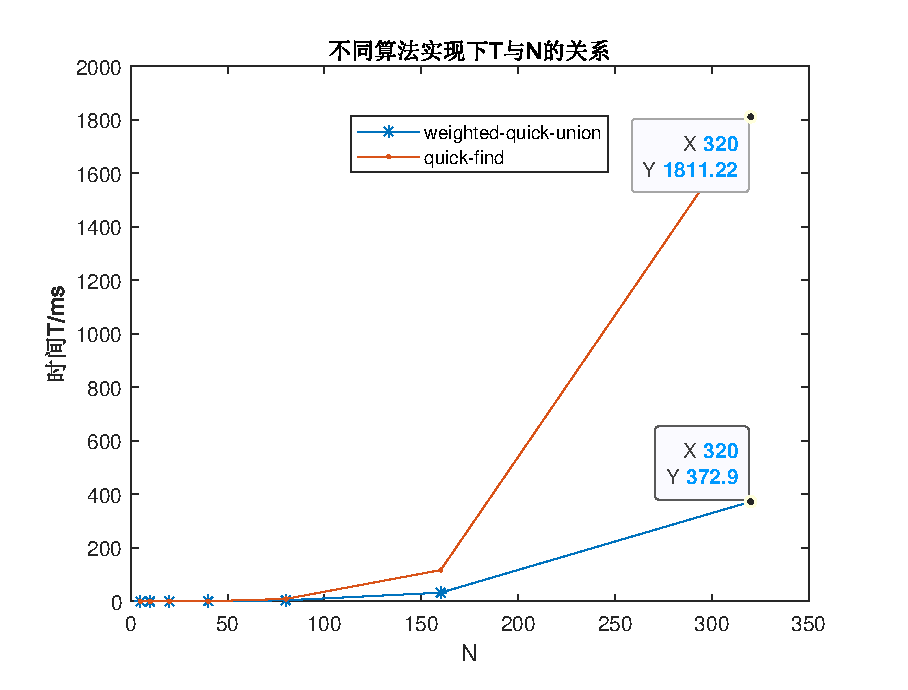
\includegraphics{percolation.eps}
    \caption{不同算法实现下T与N的关系}
\end{figure}

\paragraph{分析}从图表中可以看出,当$N>100$时,\textit{weighted-quick-union}和\textit{quick-find}时间差距
较大,这表明当 $N$ 较大时,\textit{weighted-quick-union}的效率比较高,这符合之前理论分析的时间复杂度。
\paragraph{理论估算} 由于$N \times N$ 的原因,对于\textit{weighted-quick-union}
算法,换算后的时间复杂度为
\begin{equation}
    \nonumber
    \mathcal{O}(N^2 \log{N})
\end{equation}
对于\textit{quick-find}算法来说,换算后的时间复杂度为
\begin{equation}
    \nonumber
    \mathcal{O}(N^4)
\end{equation}


通过使用\textit{Curve Fitting Tools}工具箱,通过近似计算,分别对两种算法$T$与$N$的关系进行拟合
得到函数表达式,并计算出$R^2$
\paragraph{weighted-quick-union算法下T与N的关系:}
$$ T = 0.0057 \times N^2 + -0.6942 \times N + 10.9447$$
$$ R^2 = 0.9959 $$
\paragraph{quick-find算法下T与N的关系:}
$$ T = 0.0001 \times N^3 -0.0168 \times N^2 +1.0031 \times N -15.3375$$
$$ R^2 = 1$$



\section{收获}
\begin{enumerate}
    \item[(1)] 了解并实现了\textit{weighted-quick-union}和\textit{quick-find}
    并且能够结合实际问题调用这两个算法
    \item[(2)] 认识到在数据较大时,算法的效率非常重要,尽可能选择效率较高的算法
    \item[(3)] 学会如何对两种不同的算法进行性能测试与比较,并且与理论相结合,更加深刻地理解了时间复杂度
    \item[(4)] 要合理设计不同的Java类,方便各种维度的性能测试 
\end{enumerate}

\end{document}